\begin{frame}{Spannbäume – Beispiel Kruskal}
	\centering
	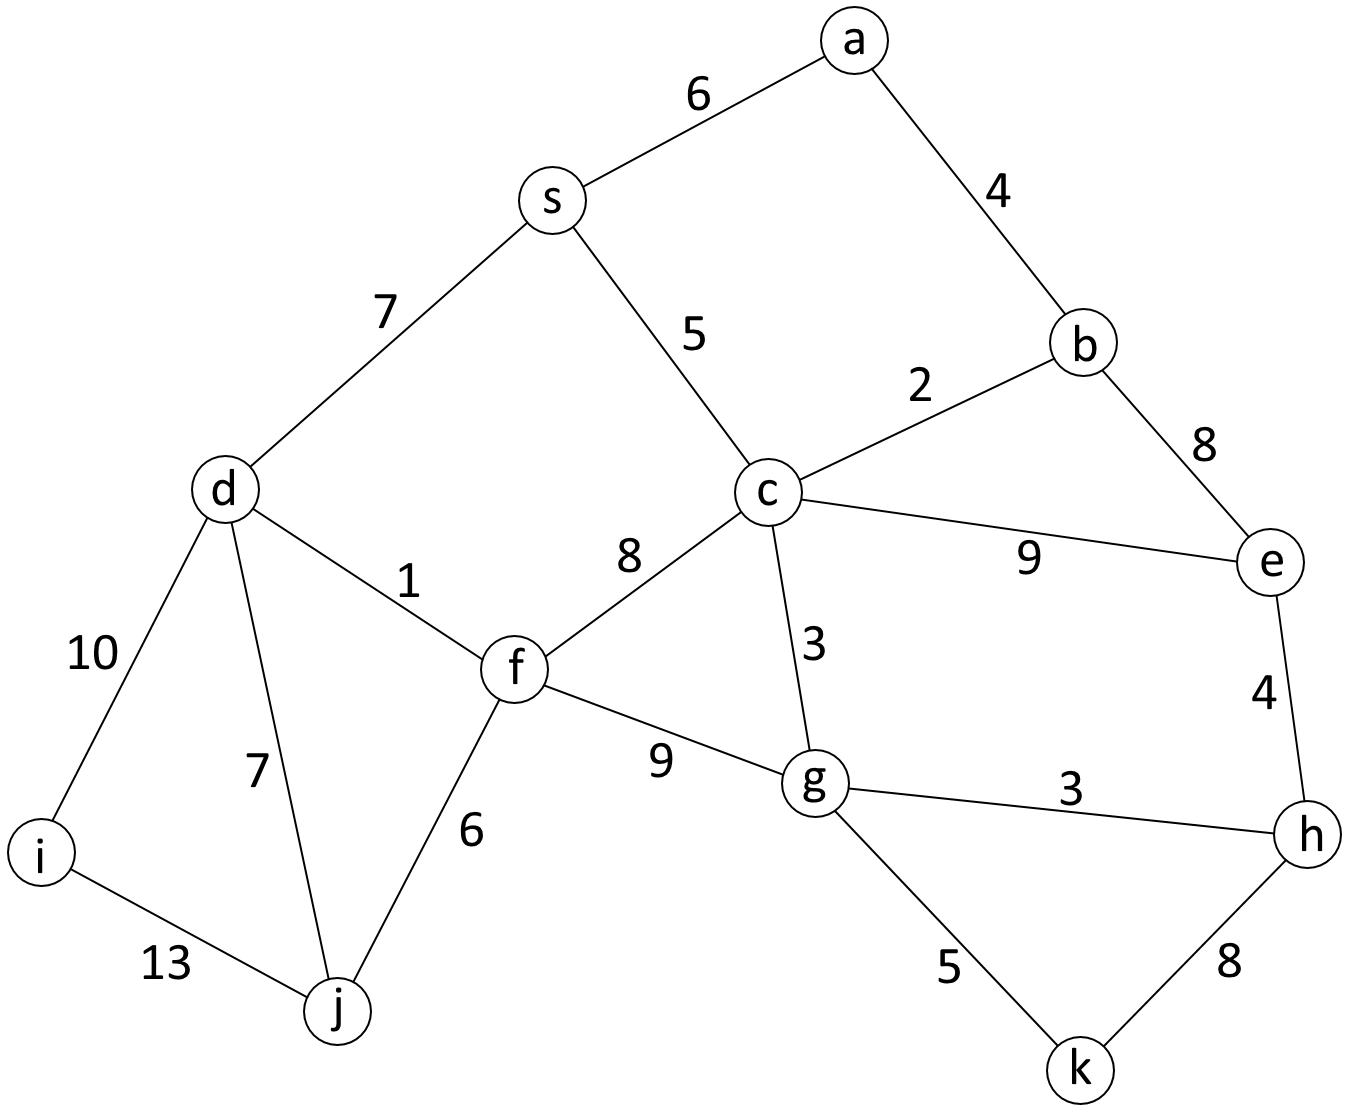
\includegraphics[width=.75\textwidth]{beispielgraph} \\
	\vspace{-.3\baselineskip}\hyperlink{label:afterEx2}{Hier klicken, um das Beispiel zu überspringen.}
\end{frame}

\begin{frame}{Spannbäume – Beispiel Kruskal}
	\centering
	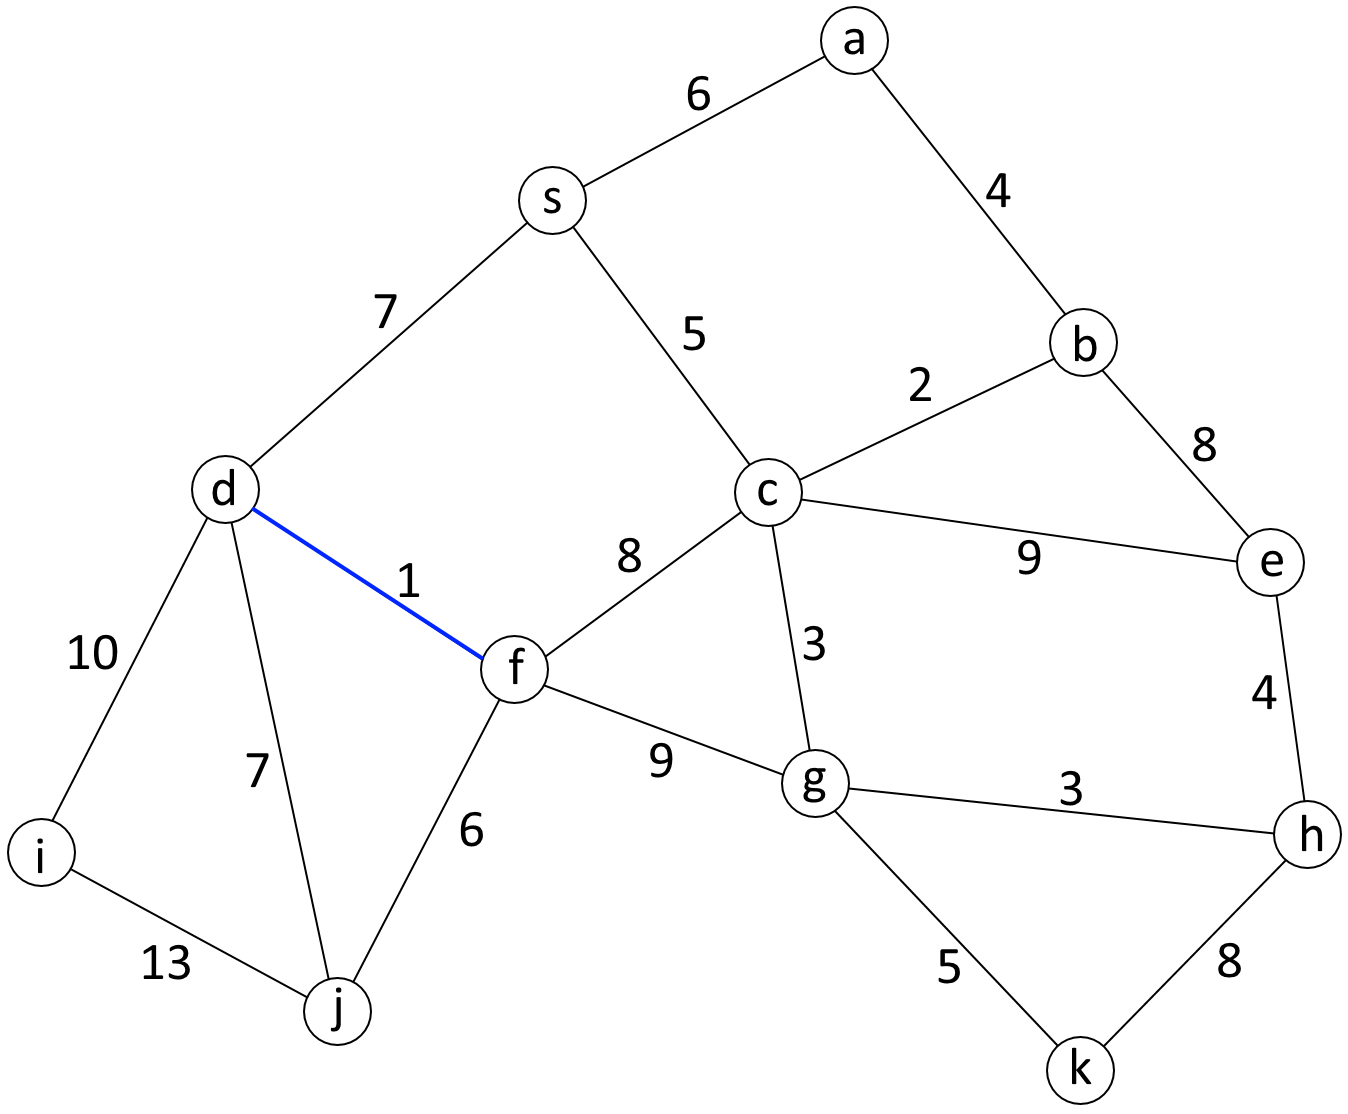
\includegraphics[width=.75\textwidth]{k1}
\end{frame}

\begin{frame}{Spannbäume – Beispiel Kruskal}
	
		\centering
		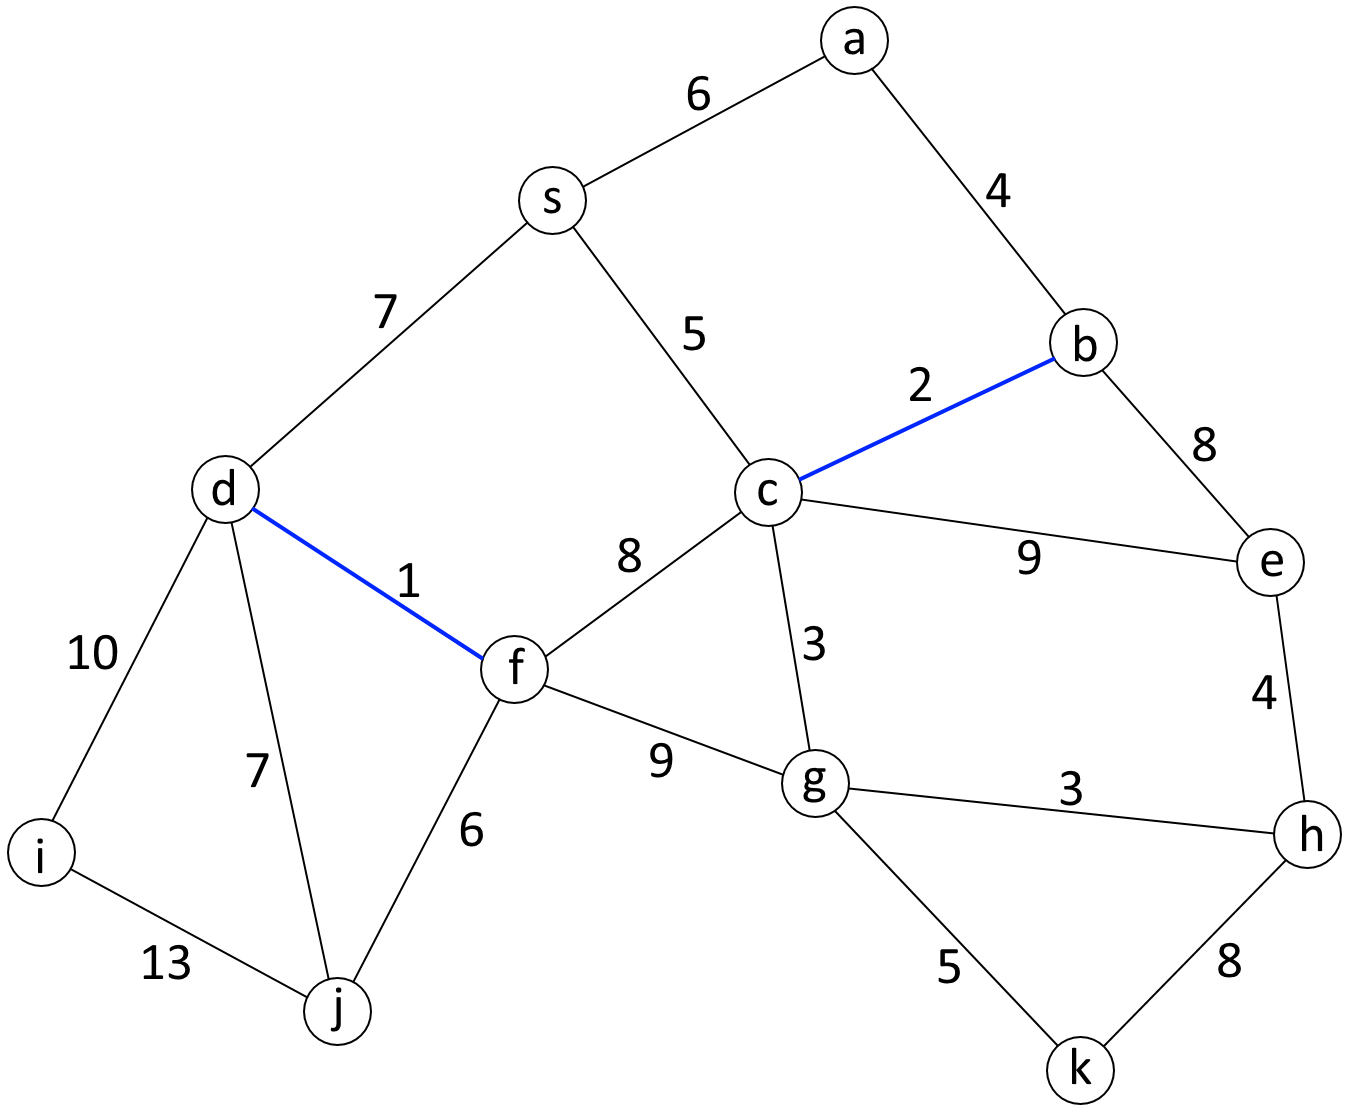
\includegraphics[width=.75\textwidth]{k2}
	
\end{frame}

\begin{frame}{Spannbäume – Beispiel Kruskal}
	
		\centering
		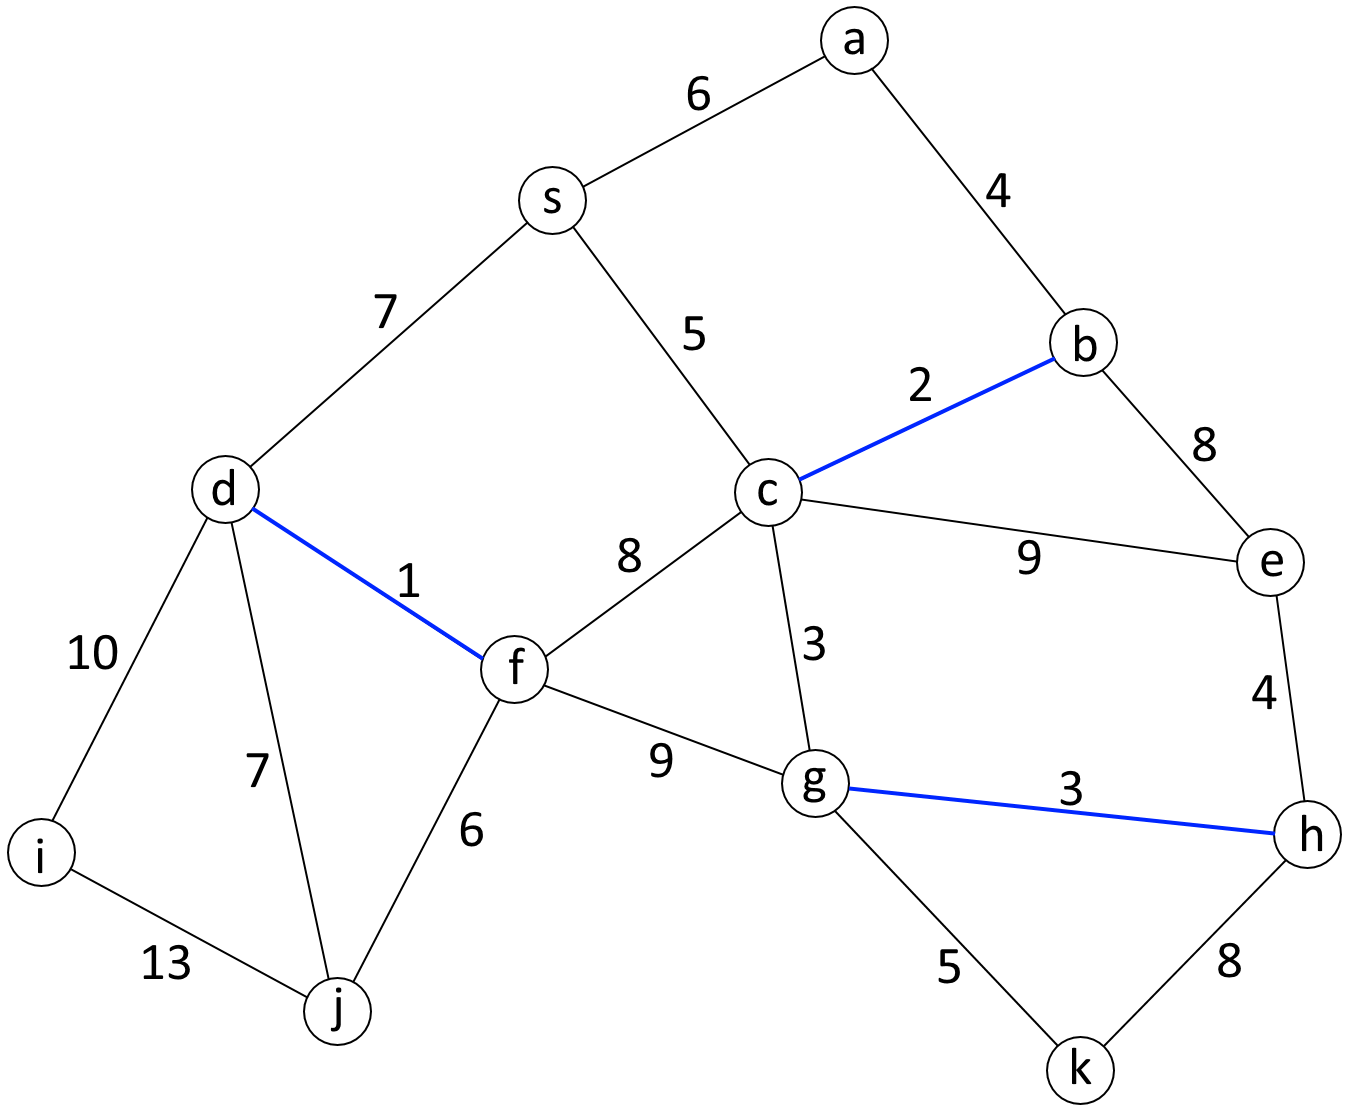
\includegraphics[width=.75\textwidth]{k3}
	
\end{frame}

\begin{frame}{Spannbäume – Beispiel Kruskal}
	
		\centering
		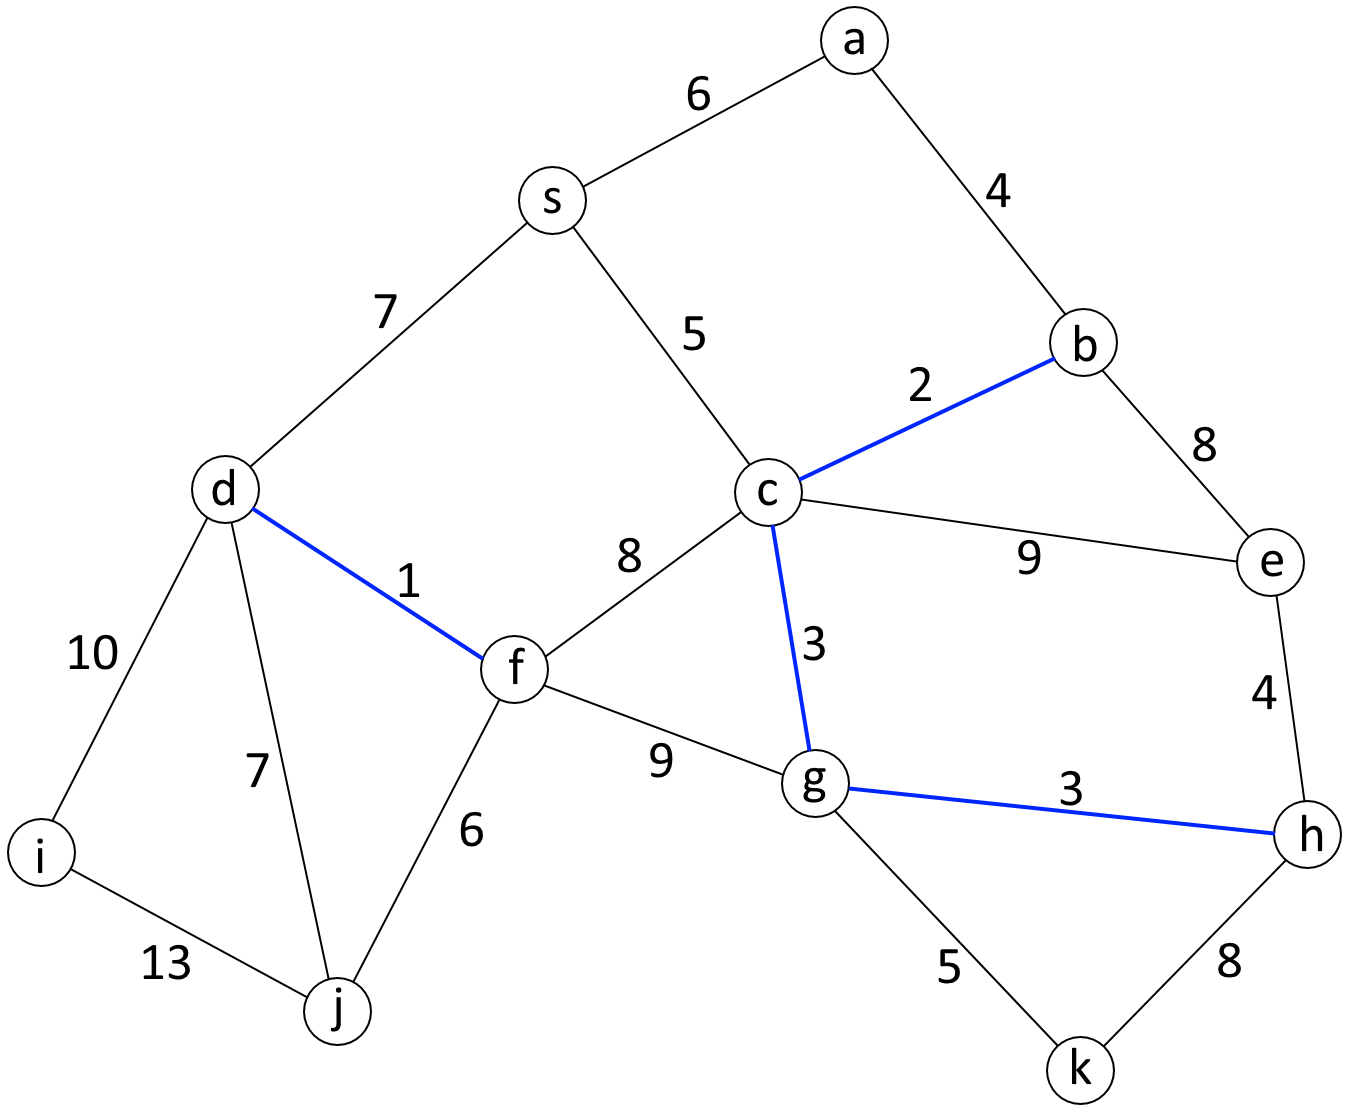
\includegraphics[width=.75\textwidth]{k4}
	
\end{frame}

\begin{frame}{Spannbäume – Beispiel Kruskal}
	
		\centering
		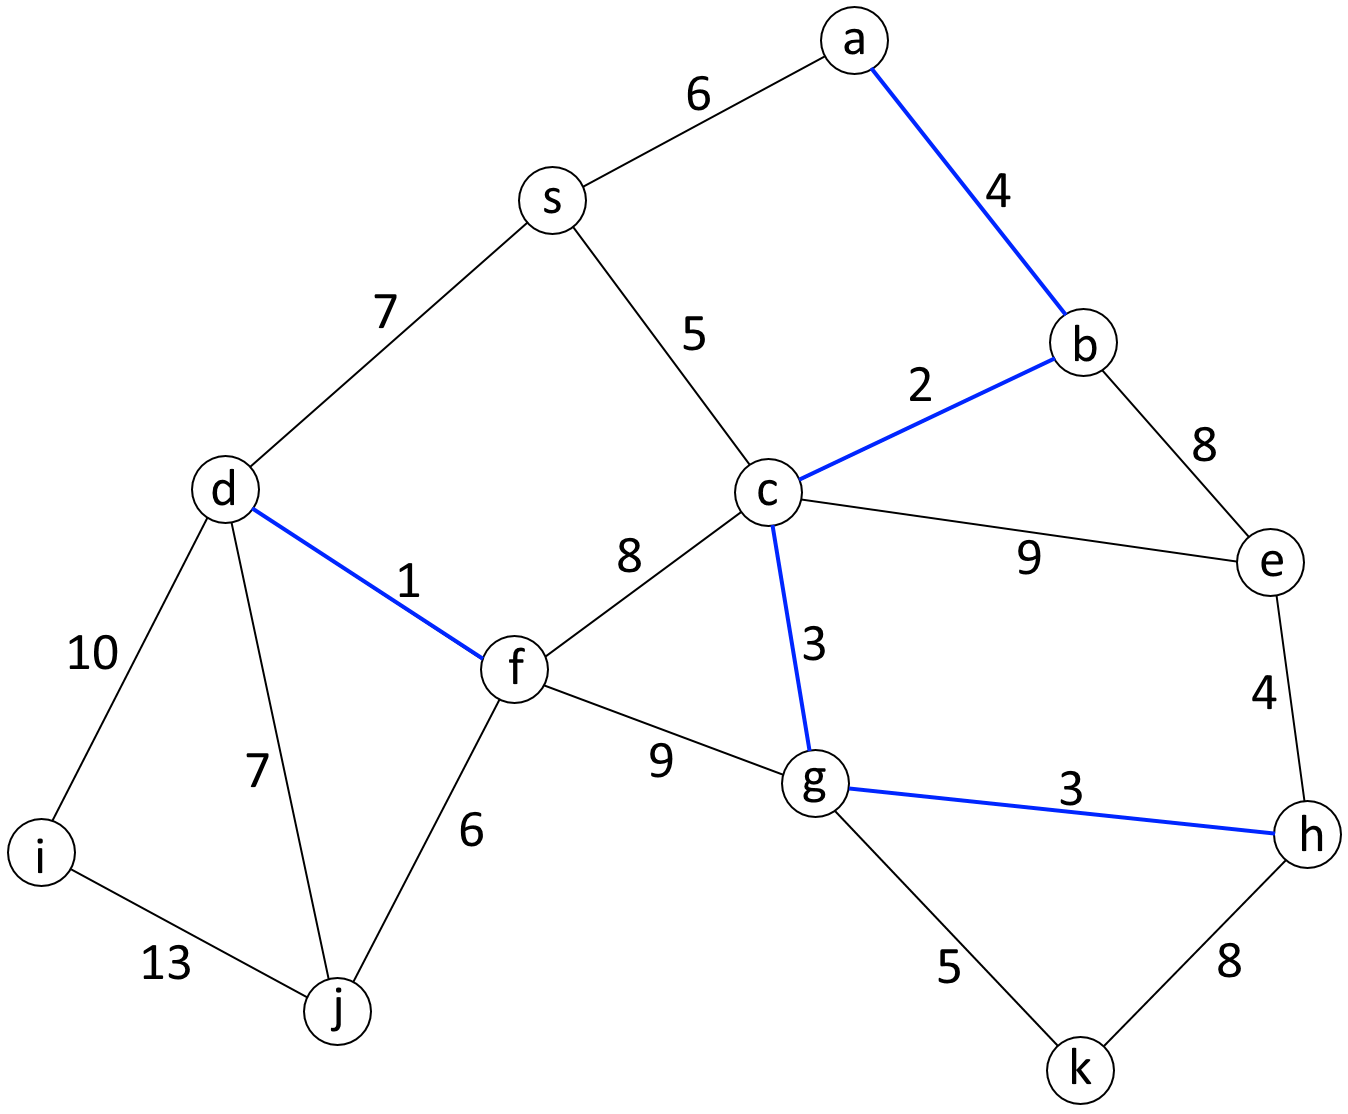
\includegraphics[width=.75\textwidth]{k5}
	
\end{frame}

\begin{frame}{Spannbäume – Beispiel Kruskal}
	
		\centering
		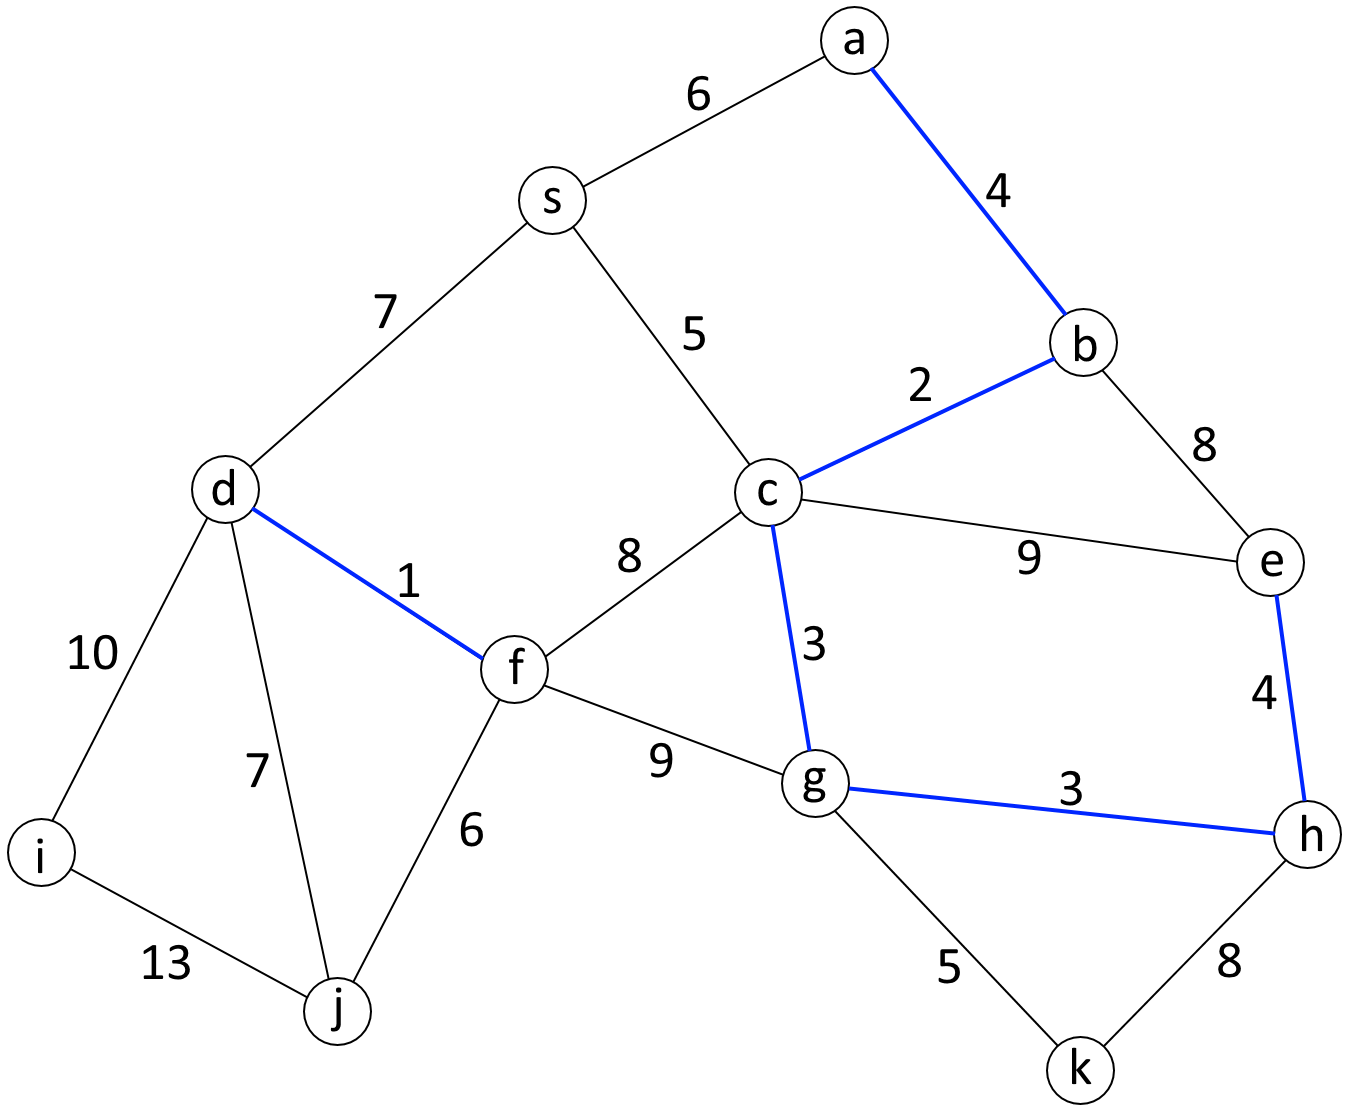
\includegraphics[width=.75\textwidth]{k6}
	
\end{frame}

\begin{frame}{Spannbäume – Beispiel Kruskal}
	
		\centering
		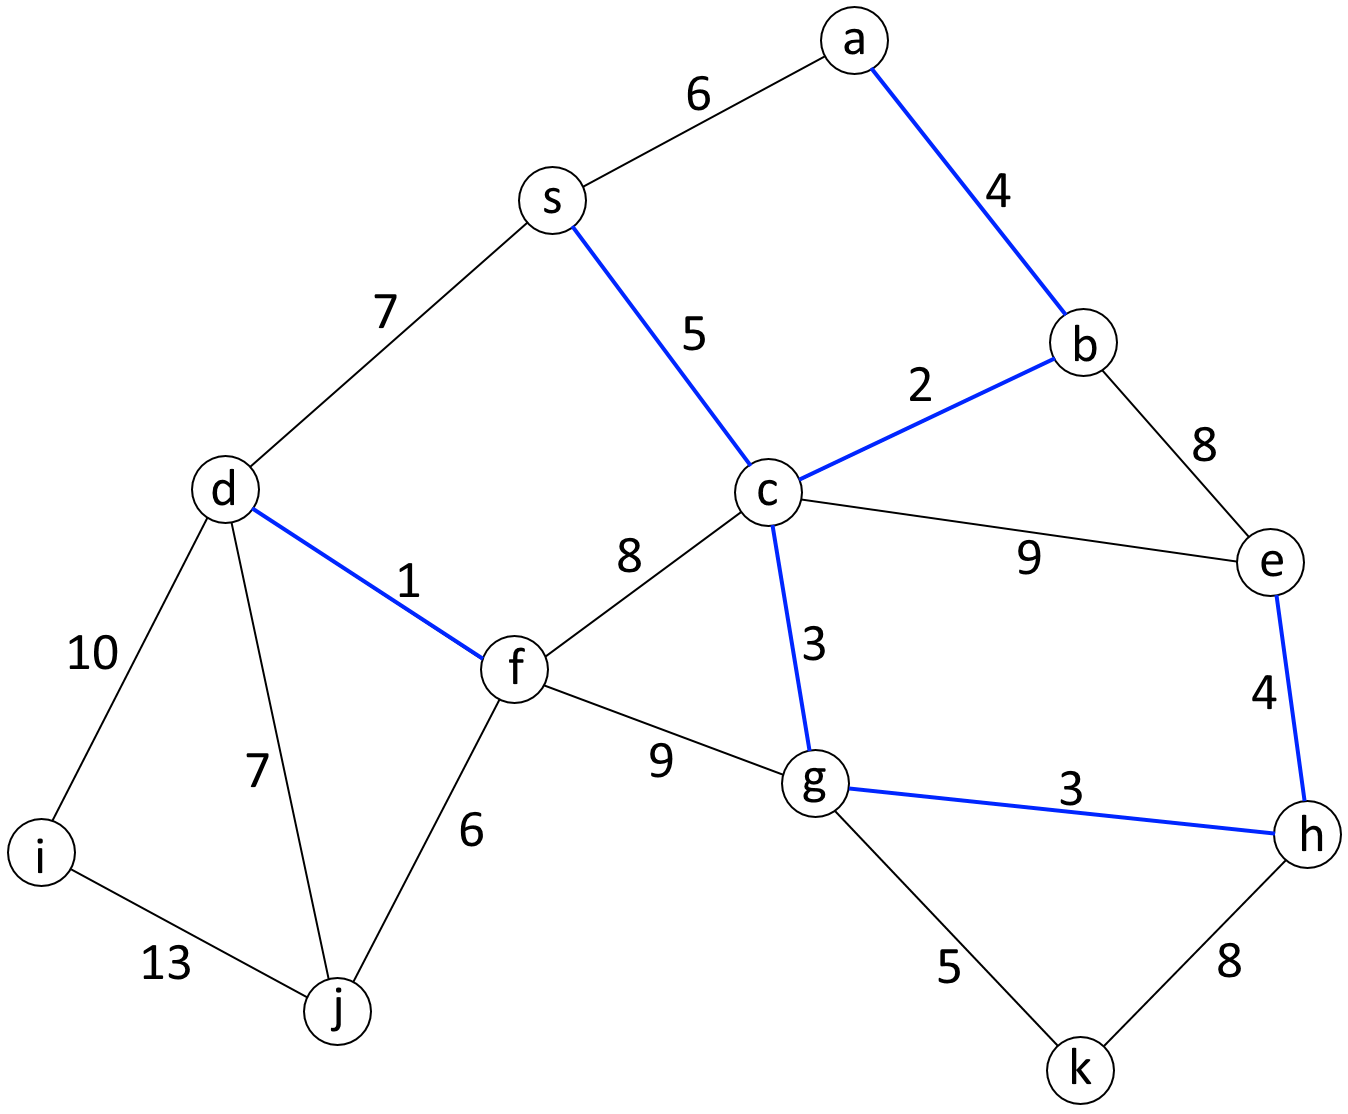
\includegraphics[width=.75\textwidth]{k7}
	
\end{frame}

\begin{frame}{Spannbäume – Beispiel Kruskal}
	
		\centering
		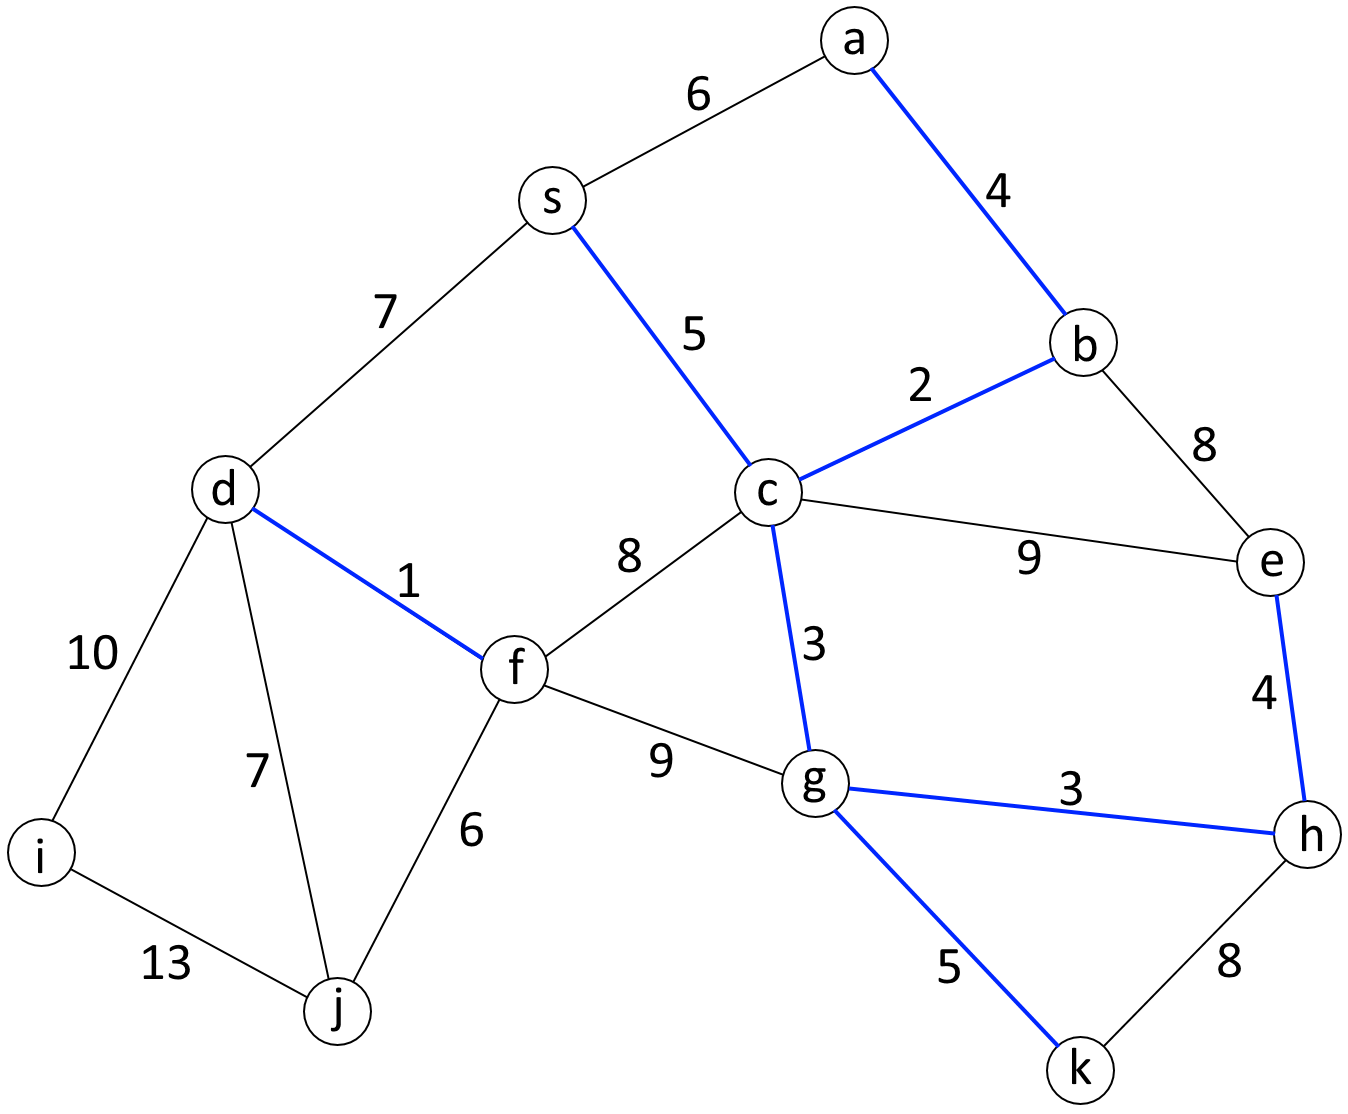
\includegraphics[width=.75\textwidth]{k8}
	
\end{frame}

\begin{frame}{Spannbäume – Beispiel Kruskal}
	
		\centering
		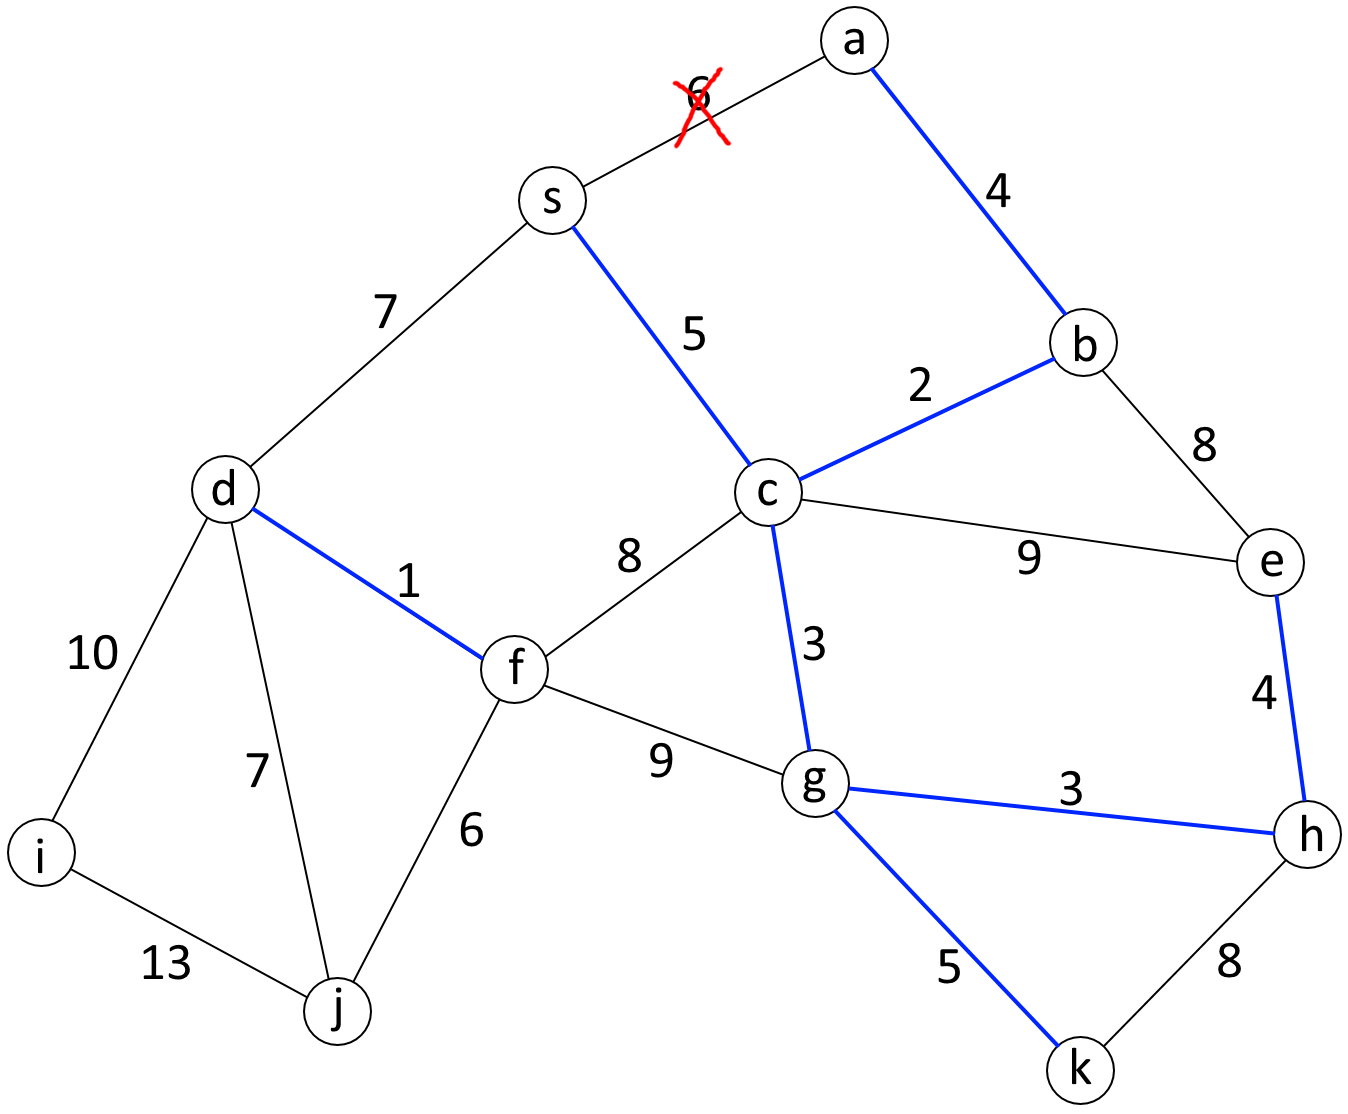
\includegraphics[width=.75\textwidth]{k9}
	
\end{frame}

\begin{frame}{Spannbäume – Beispiel Kruskal}
	
		\centering
		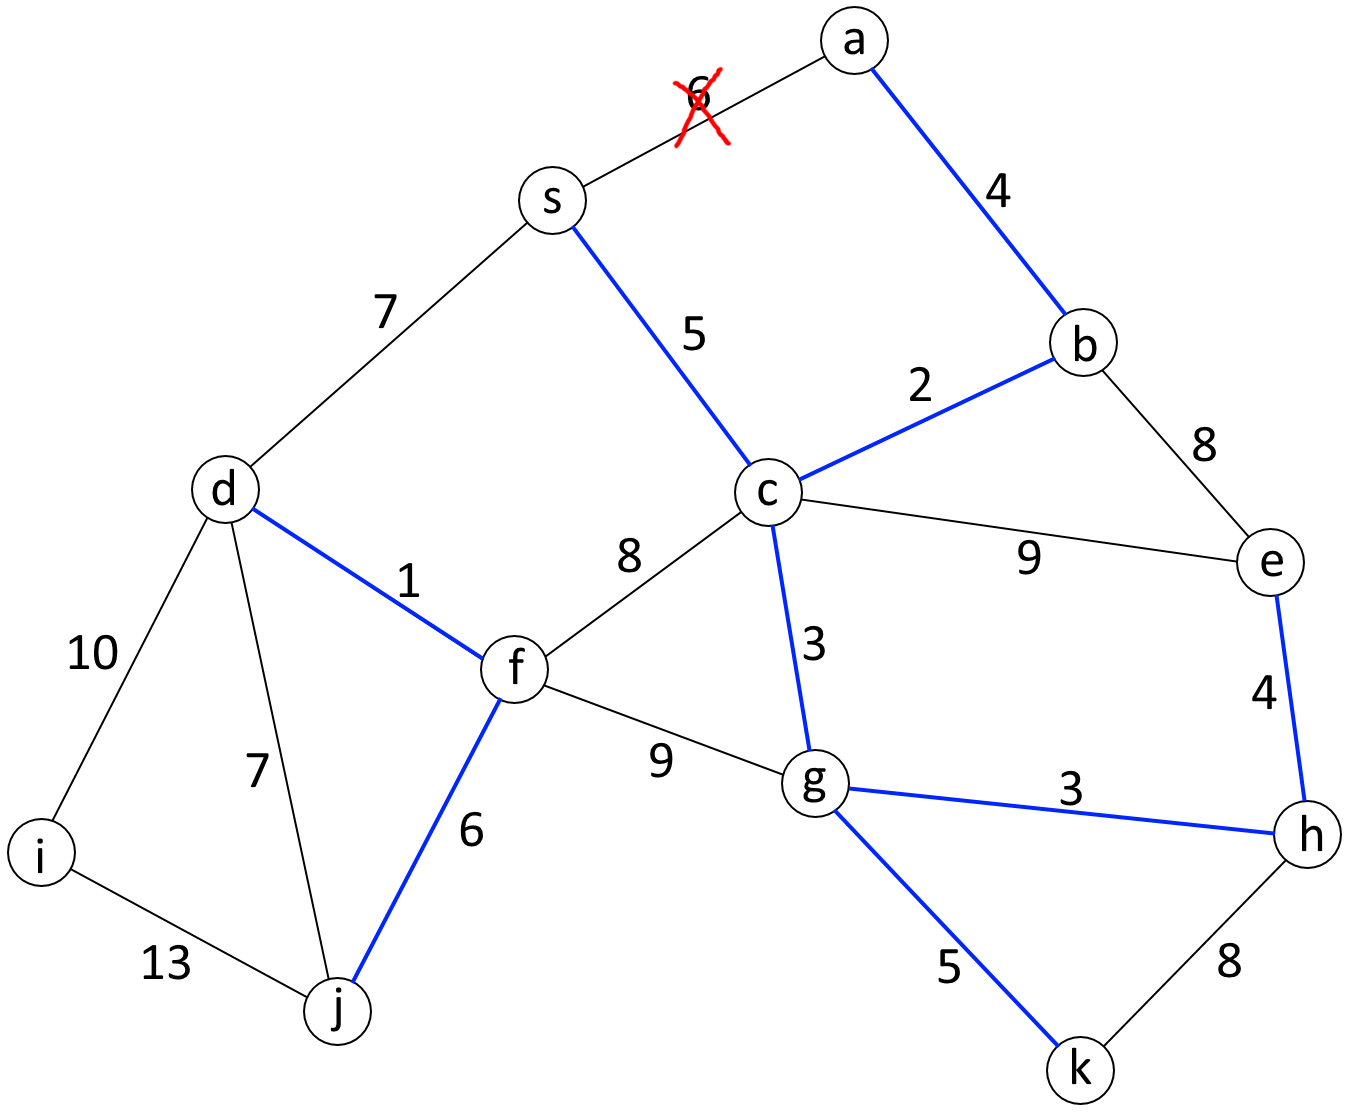
\includegraphics[width=.75\textwidth]{k10}
	
\end{frame}

\begin{frame}{Spannbäume – Beispiel Kruskal}
	
		\centering
		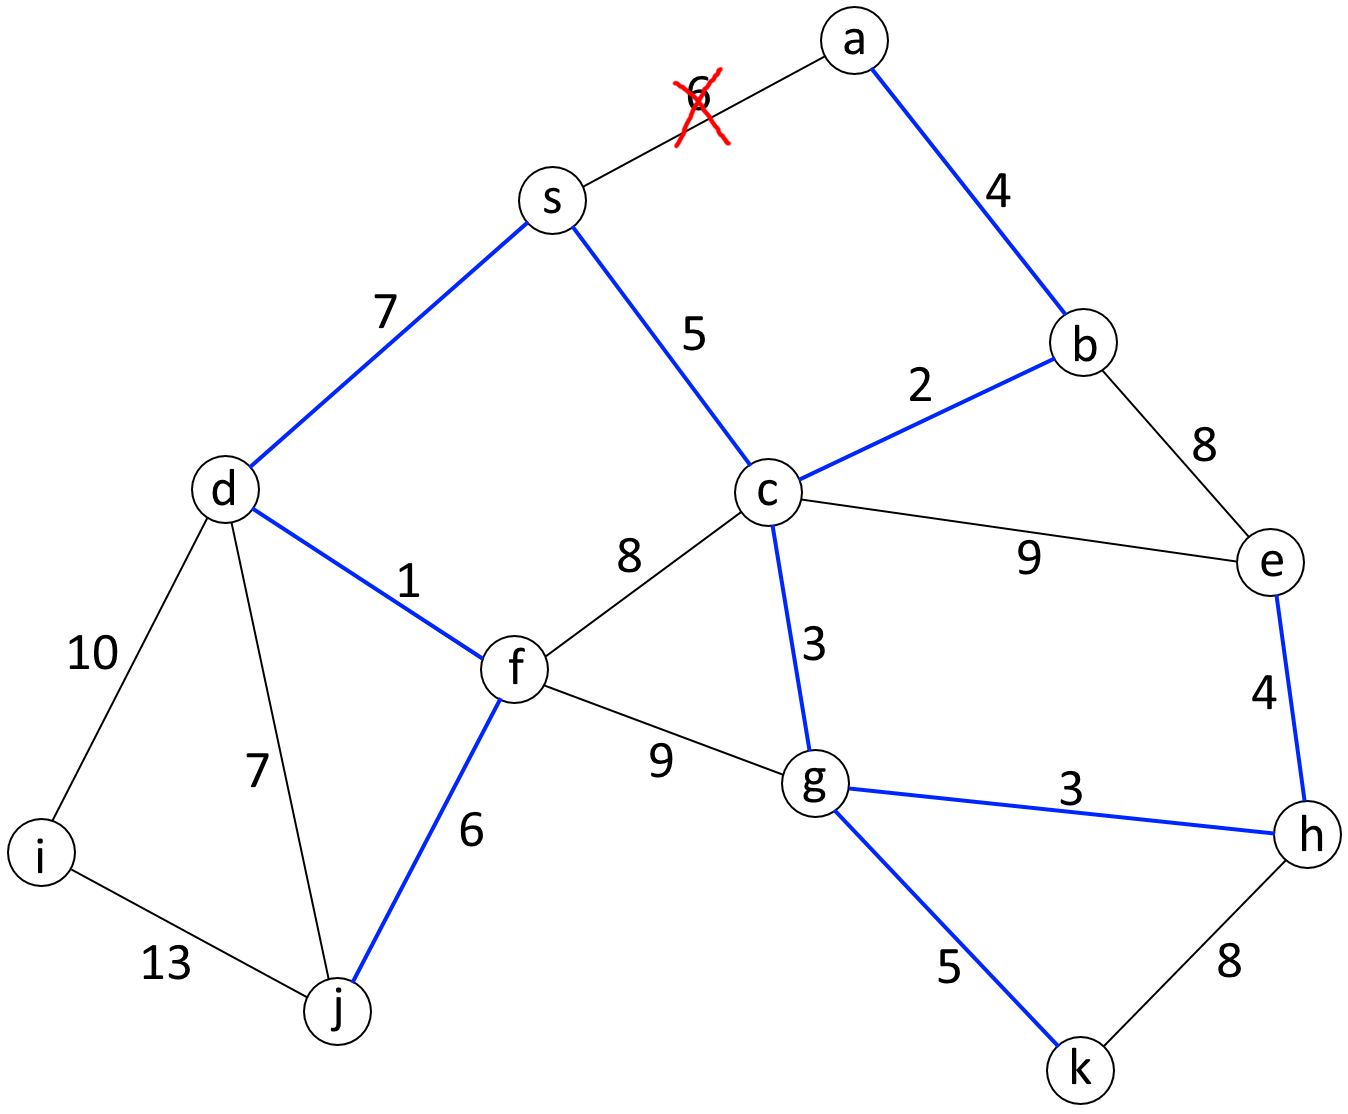
\includegraphics[width=.75\textwidth]{k11}
	
\end{frame}

\begin{frame}{Spannbäume – Beispiel Kruskal}
	
		\centering
		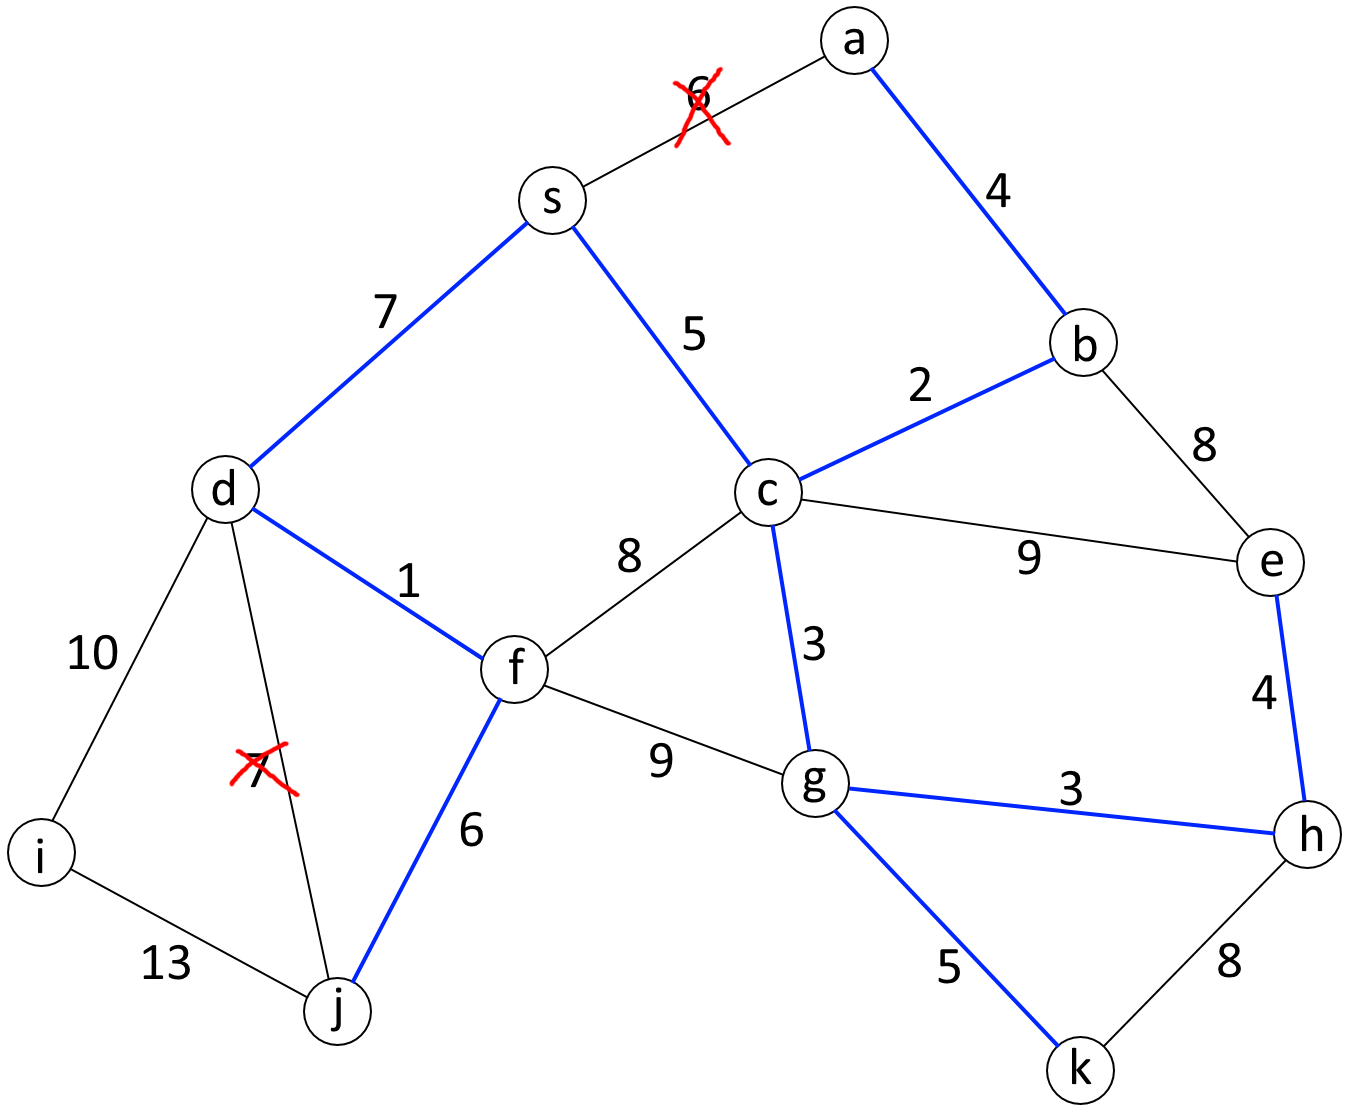
\includegraphics[width=.75\textwidth]{k12}
	
\end{frame}

\begin{frame}{Spannbäume – Beispiel Kruskal}
	
		\centering
		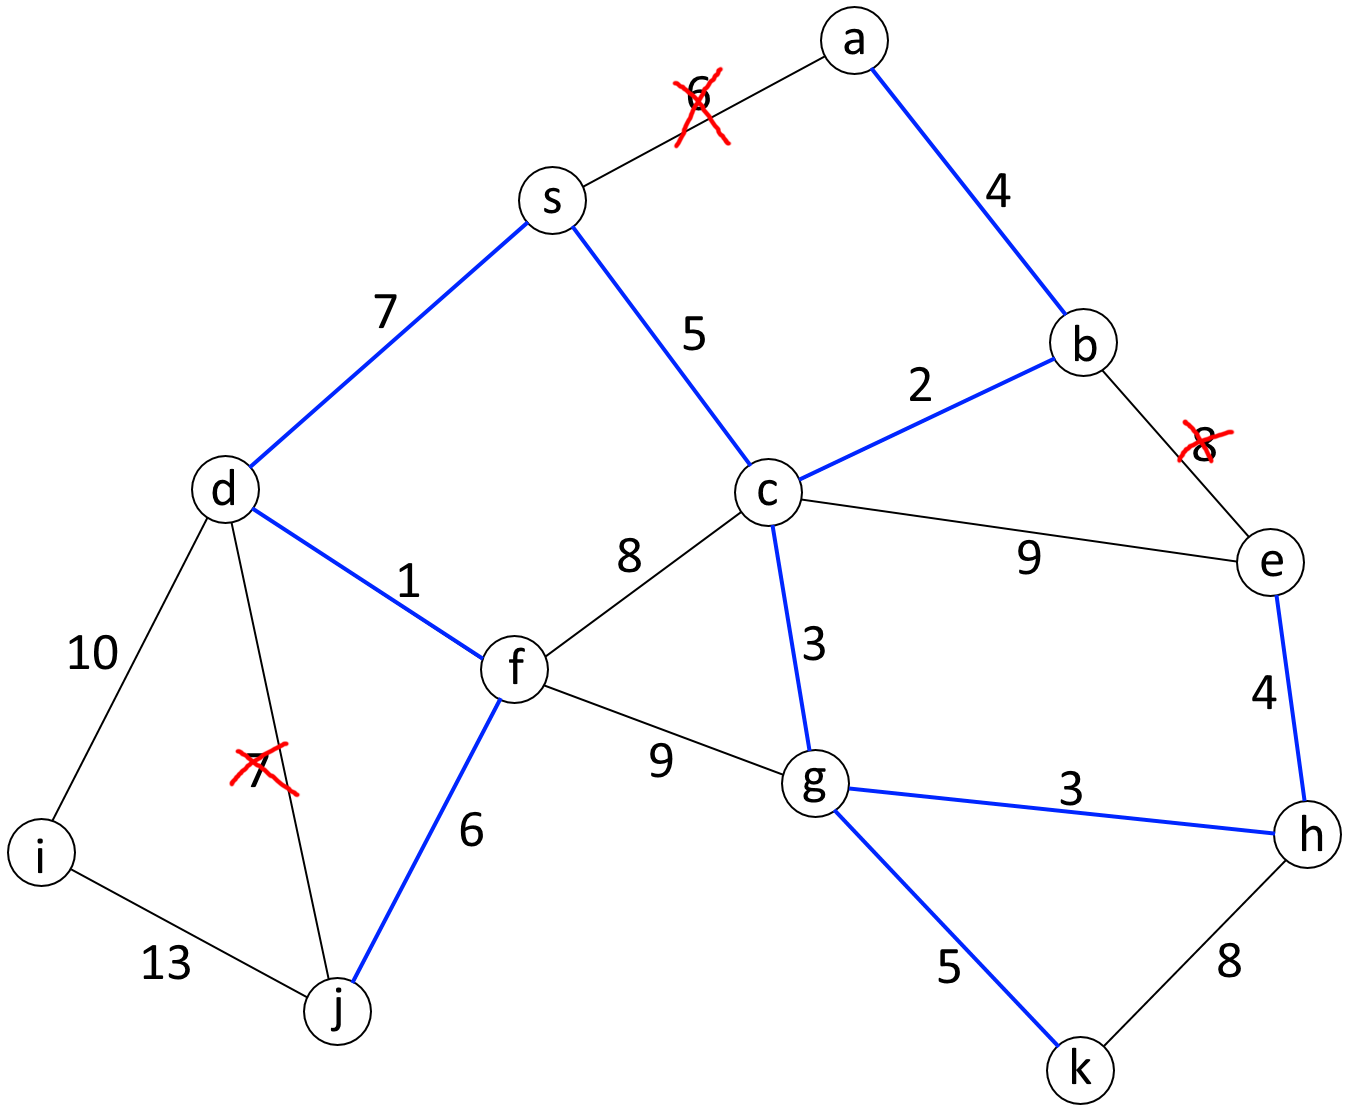
\includegraphics[width=.75\textwidth]{k13}
	
\end{frame}

\begin{frame}{Spannbäume – Beispiel Kruskal}
	
		\centering
		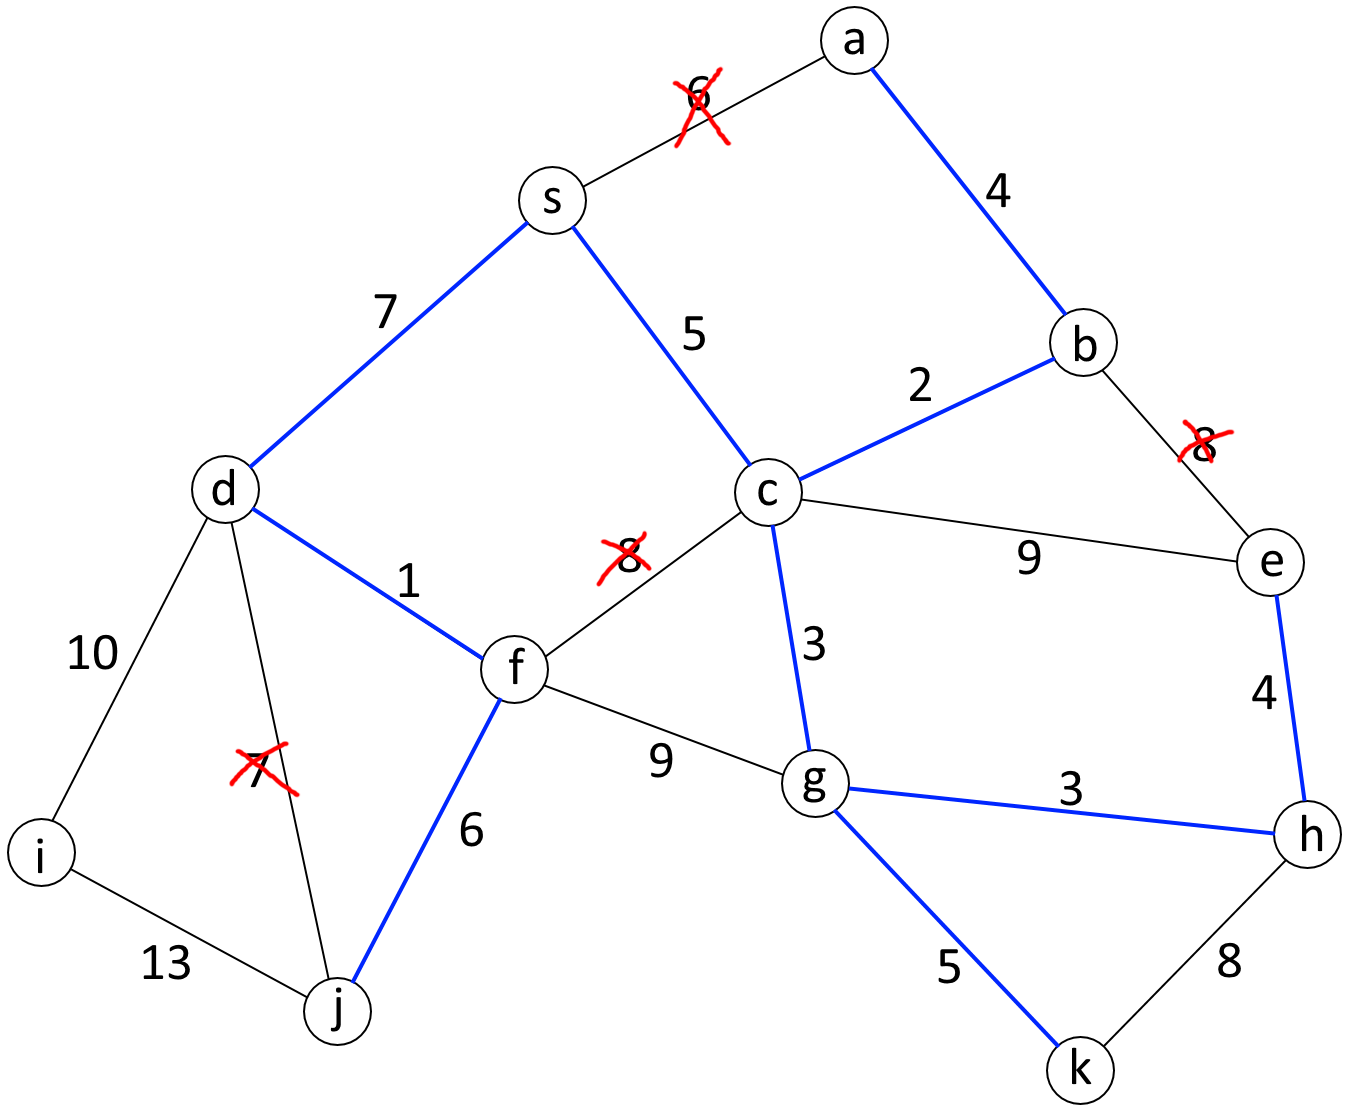
\includegraphics[width=.75\textwidth]{k14}
	
\end{frame}

\begin{frame}{Spannbäume – Beispiel Kruskal}
	
		\centering
		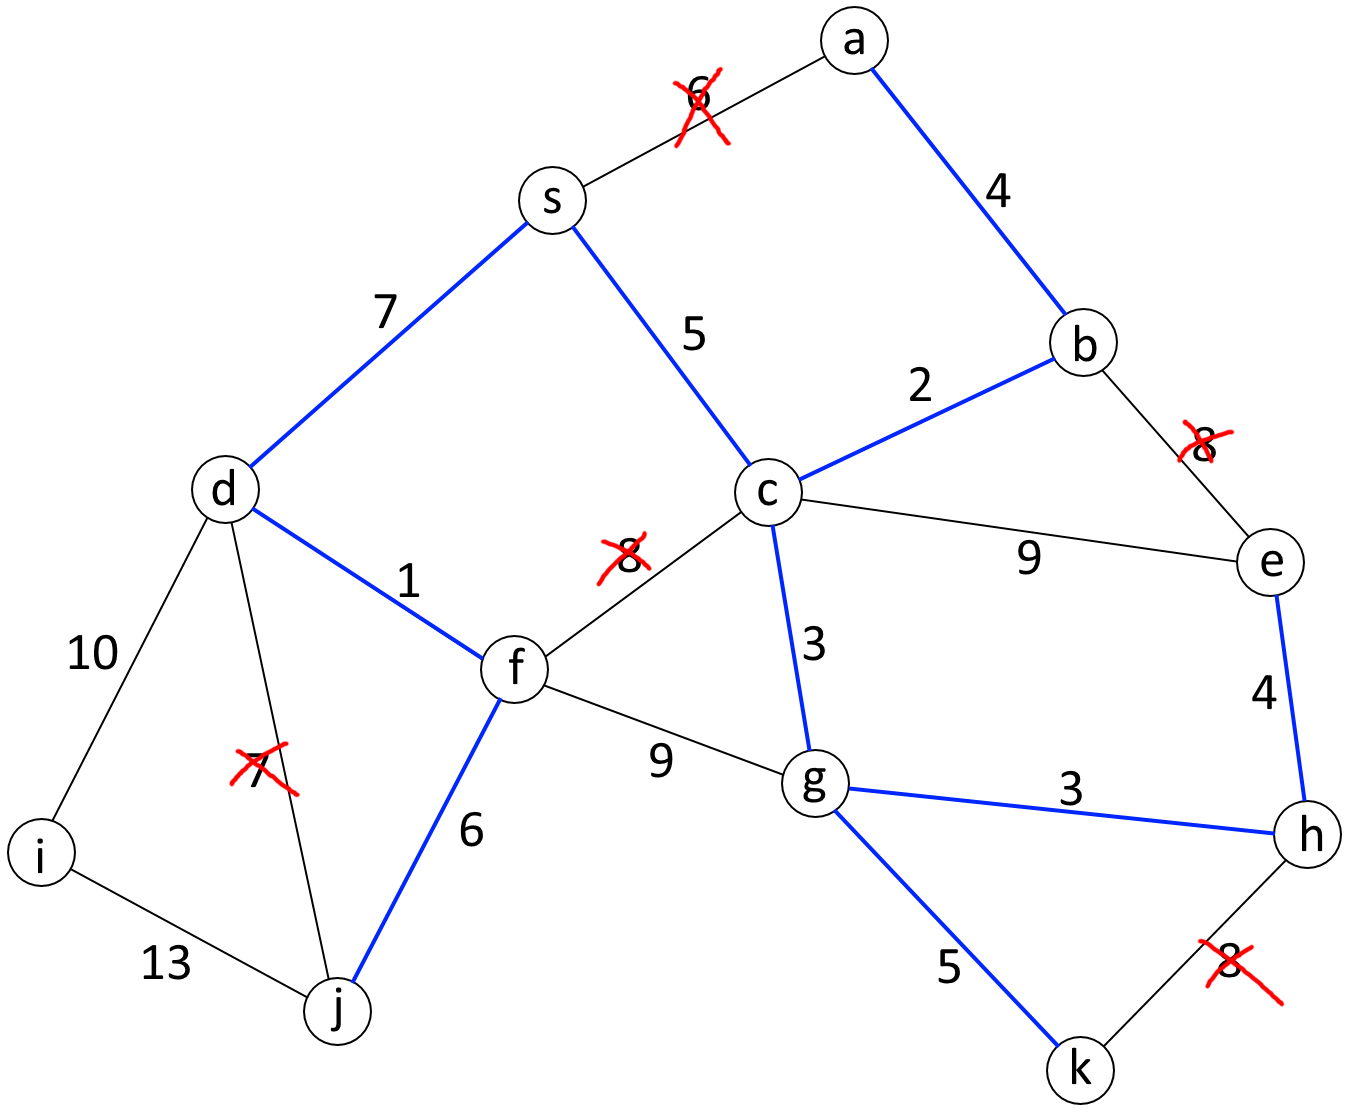
\includegraphics[width=.75\textwidth]{k15}
	
\end{frame}

\begin{frame}{Spannbäume – Beispiel Kruskal}
	
		\centering
		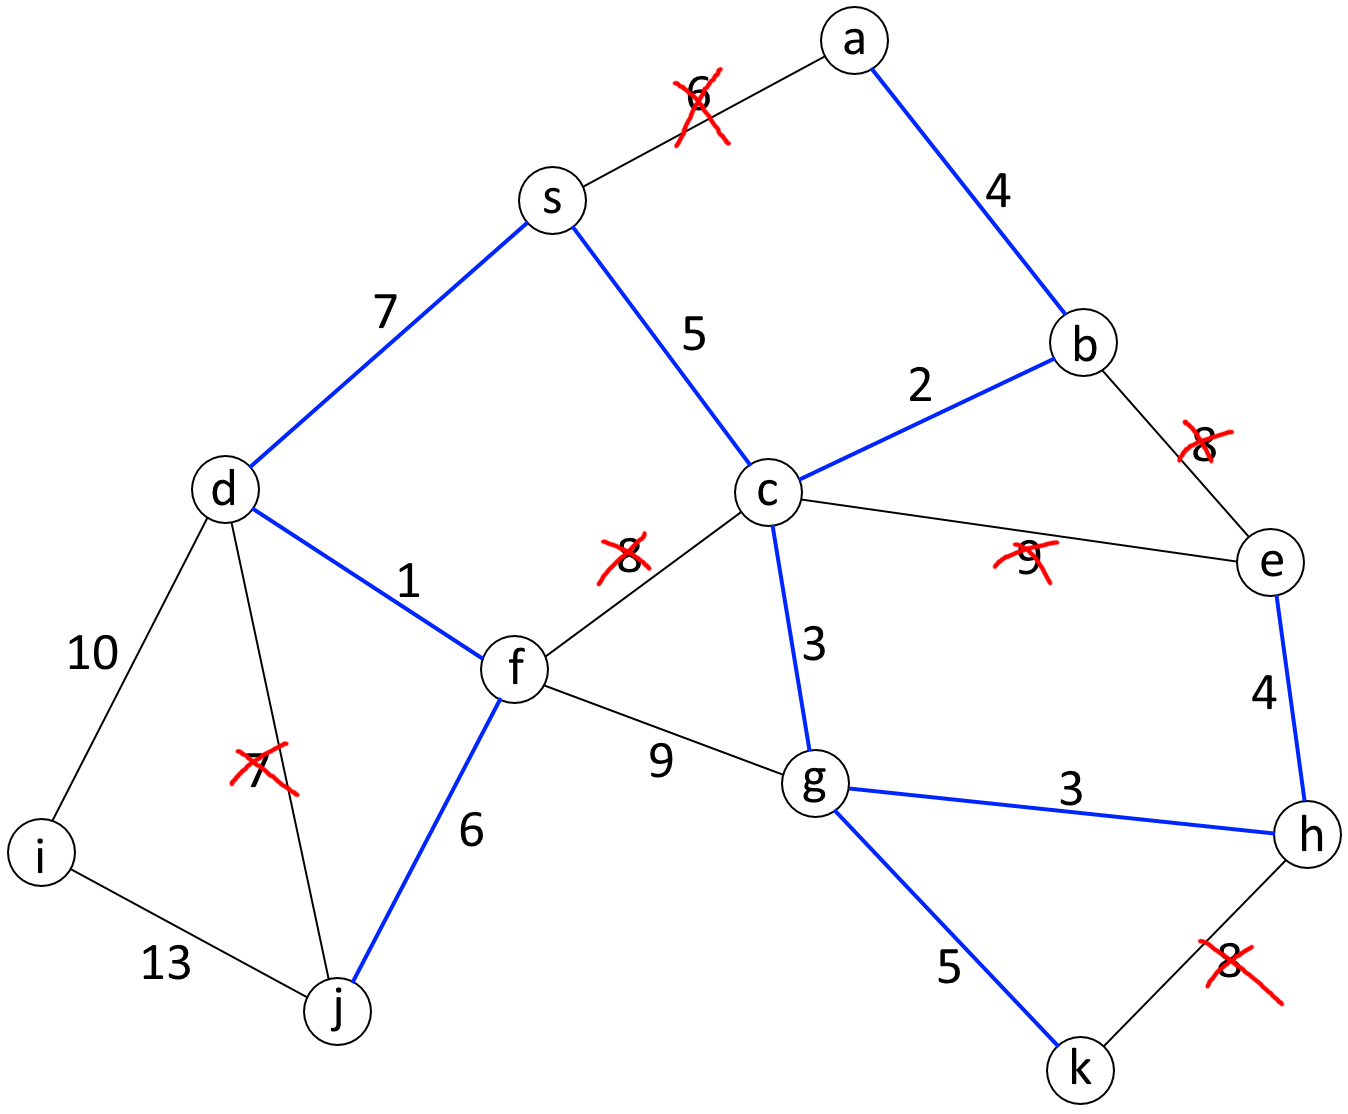
\includegraphics[width=.75\textwidth]{k16}
	
\end{frame}

\begin{frame}{Spannbäume – Beispiel Kruskal}
	
		\centering
		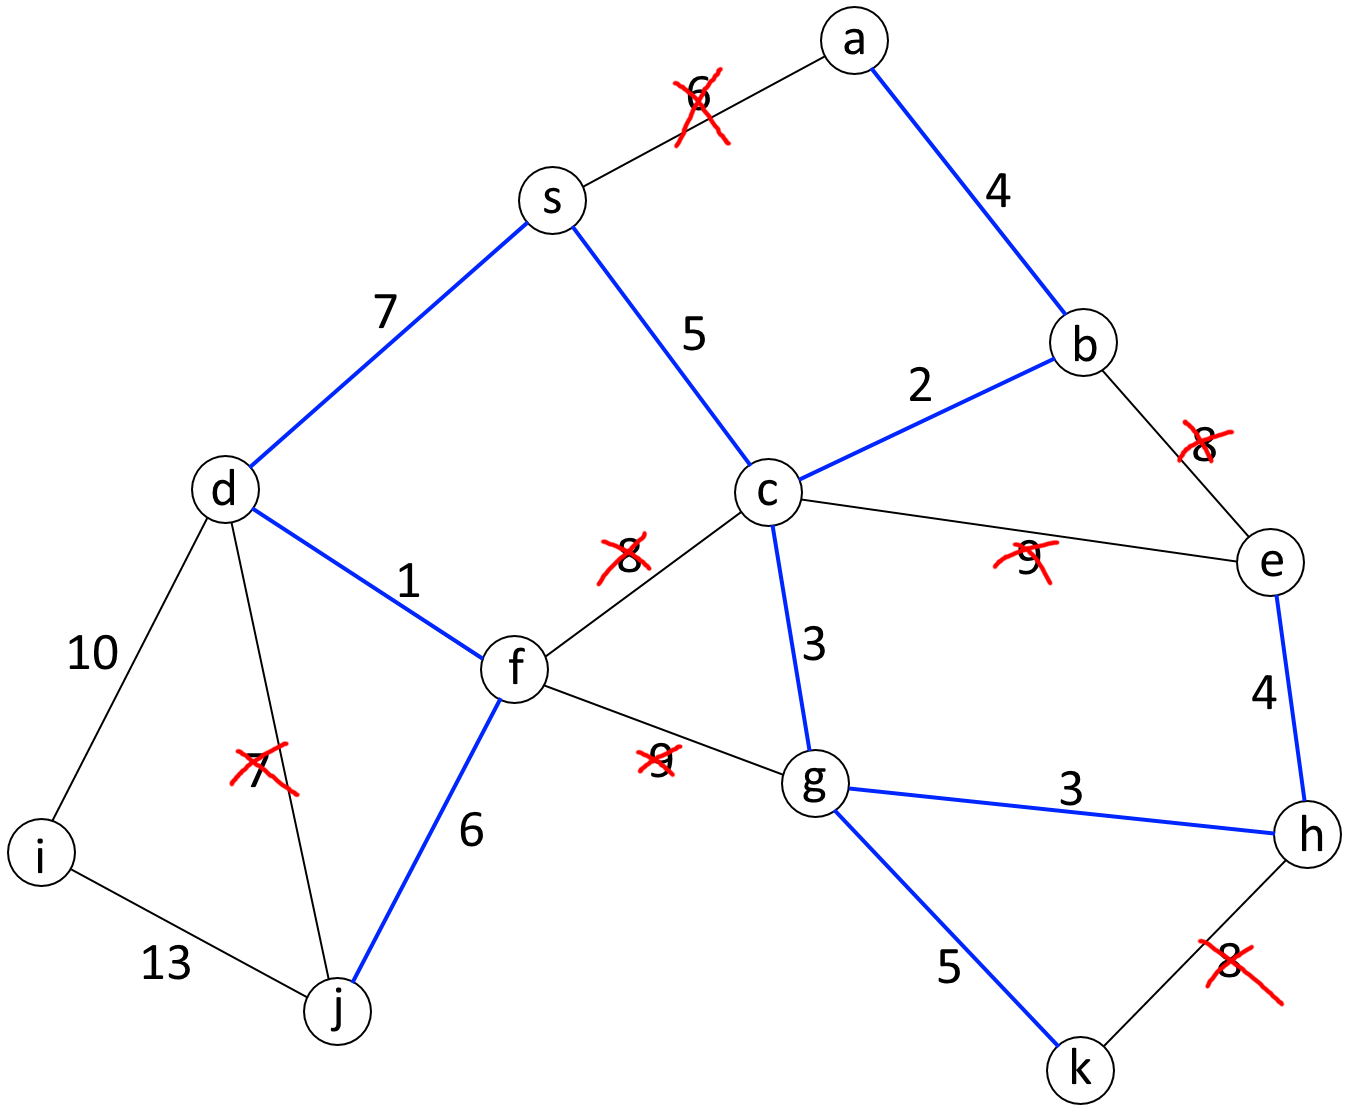
\includegraphics[width=.75\textwidth]{k17}
	
\end{frame}

\begin{frame}{Spannbäume – Beispiel Kruskal}
	
		\centering
		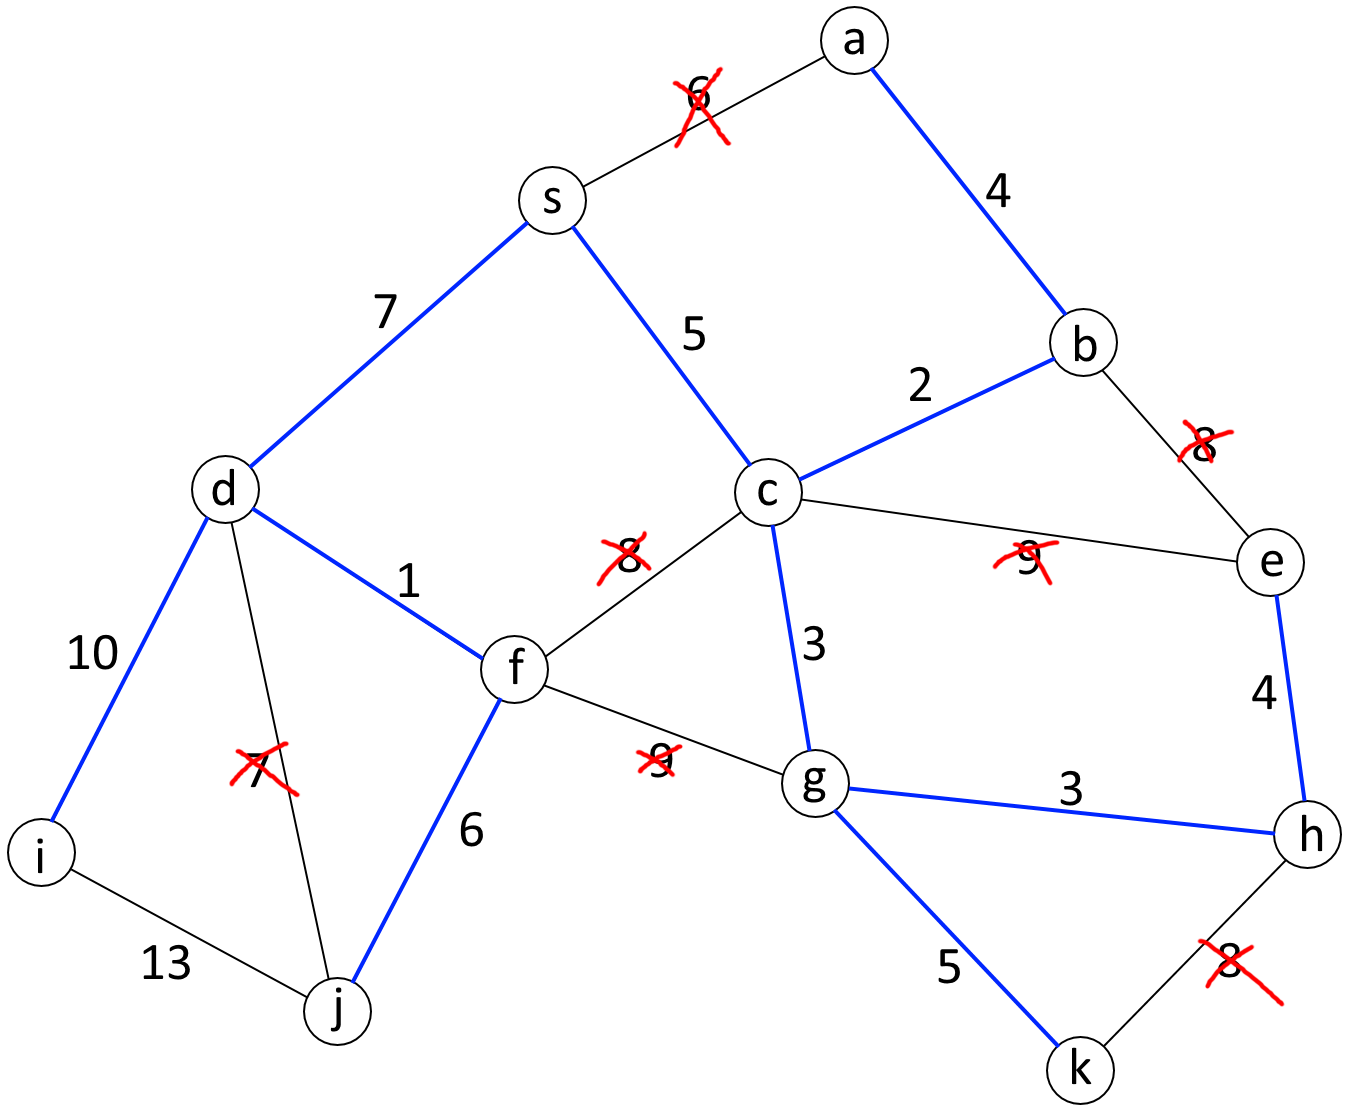
\includegraphics[width=.75\textwidth]{k18}
	
\end{frame}

\begin{frame}{\hypertarget{label:afterEx2}{}Spannbäume – Beispiel Kruskal}
		\centering
		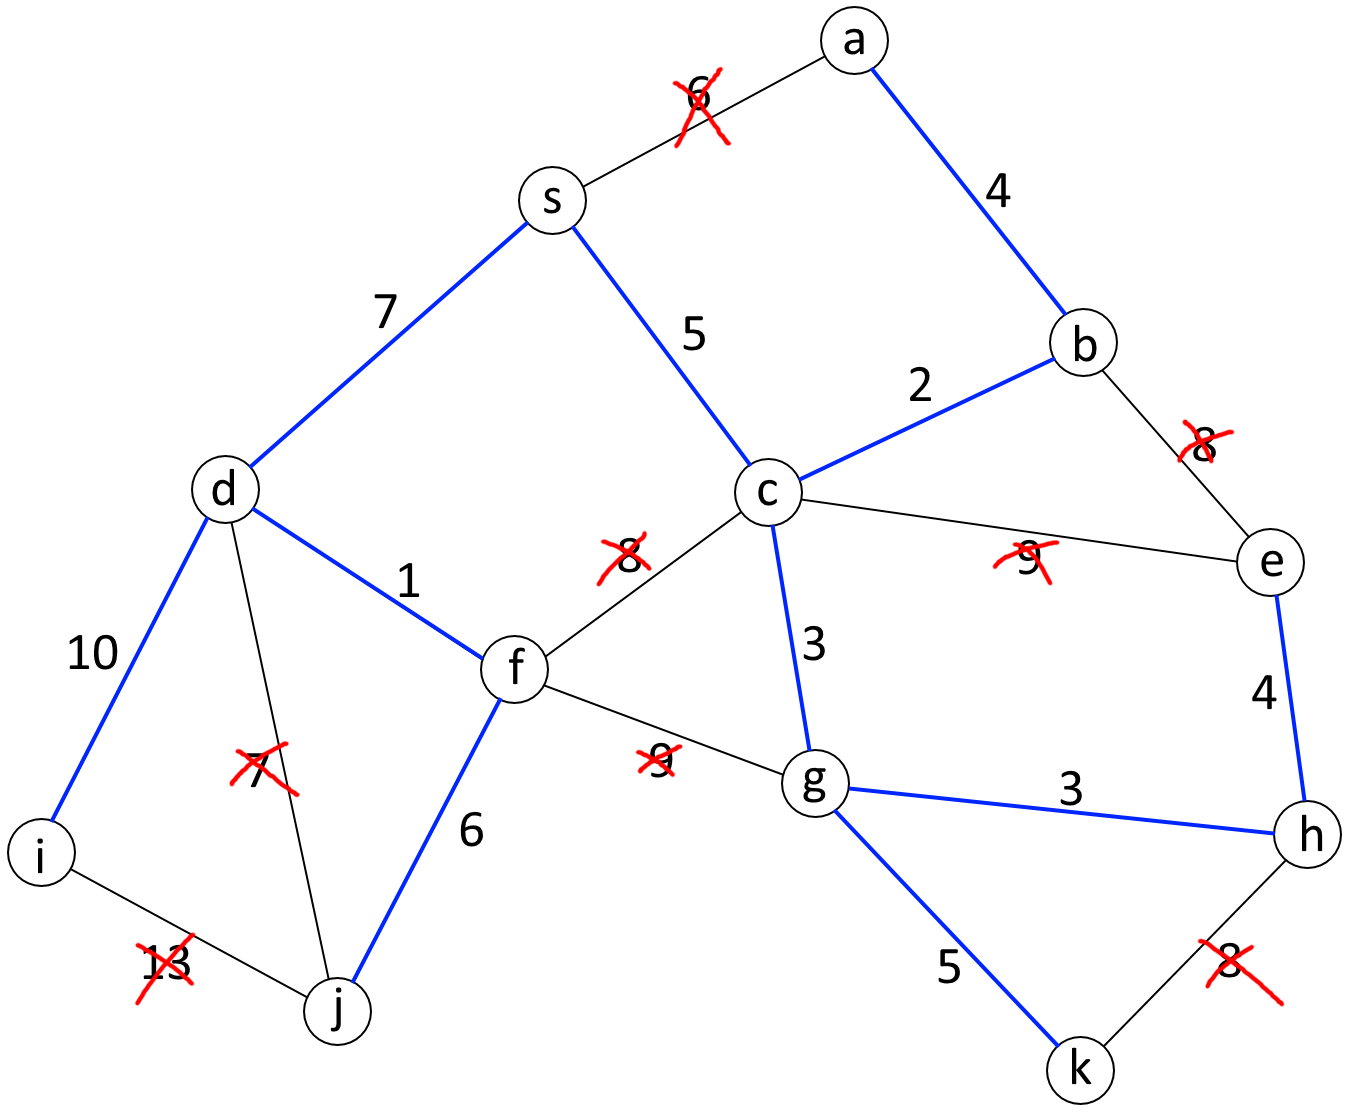
\includegraphics[width=.75\textwidth]{k19}
\end{frame}
